

\documentclass[hidelinks, 11pt, fleqn]{article}   	% use "amsart" instead of "article" for AMSLaTeX format
\usepackage{geometry}                		% See geometry.pdf to learn the layout options. There are lots.
\usepackage{tikz}
\usepackage{listings}
\usepackage{color}

\definecolor{codegreen}{rgb}{0,0.6,0}
\definecolor{codegray}{rgb}{0.5,0.5,0.5}
\definecolor{lightgray}{rgb}{0.7,0.7,0.7}
\definecolor{codepurple}{rgb}{0.58,0,0.82}
\definecolor{backcolour}{rgb}{0.92,0.92,0.92}

\renewcommand{\lstlistingname}{Algorithm}% Listing -> Algorithm

\lstdefinestyle{mystyle}{
	backgroundcolor=\color{backcolour},   
	commentstyle=\color{codegray},
	keywordstyle=\color{red},
	numberstyle=\tiny\color{lightgray},
	stringstyle=\color{codepurple},
	basicstyle=\footnotesize,
	breakatwhitespace=false,         
	breaklines=true,                 
	captionpos=b,                    
	keepspaces=true,                 
	numbers=left,                    
	numbersep=5pt,                  
	showspaces=false,                
	showstringspaces=false,
	showtabs=false,                  
	tabsize=4
}

\lstset{style=mystyle}

\usepackage{amsmath}
\usepackage{mathtools}
\usepackage{algorithm}
\usepackage{algpseudocode}
\geometry{letterpaper}                   		% ... or a4paper or a5paper or ... 
%\geometry{landscape}                		% Activate for rotated page geometry
%\usepackage[parfill]{parskip}    		% Activate to begin paragraphs with an empty line rather than an indent
\usepackage{graphicx}				% Use pdf, png, jpg, or eps§ with pdflatex; use eps in DVI mode
\usepackage{subcaption}
\usepackage{hyperref}
								% TeX will automatically convert eps --> pdf in pdflatex		
\usepackage{amssymb}

%SetFonts

%SetFonts
\newtagform{brackets}{[}{]}
\usetagform{brackets}

\title{\textbf{Generate stepper motor S-shaped motion profiles using sigmoid functions}}
\author{Patrick Sorn}
%\date{}							% Activate to display a given date or no date

\begin{document}
\maketitle
\tableofcontents 
\pagebreak
\section{Trapezoidal speed ramp}
In order to understand how stepper motor ramp profiles work, we have to dive into the most commonly used and most applicable profile type: the trapezoidal ramp profile. 
It consists of 3 phases: An acceleration phase $T_{a}$, a constant velocity phase $T_{c}$ and a deceleration phase $T_{d}$. The sum of the 3 phases constitutes the total time $T$ (see Fig. \ref{fig:trapezoid_detail}). The trapezoidal ramp profile is the simplest solution, as it can be represented by the standard physics formula for velocity with constant acceleration.
\newline
\newline
\begin{figure}[h]
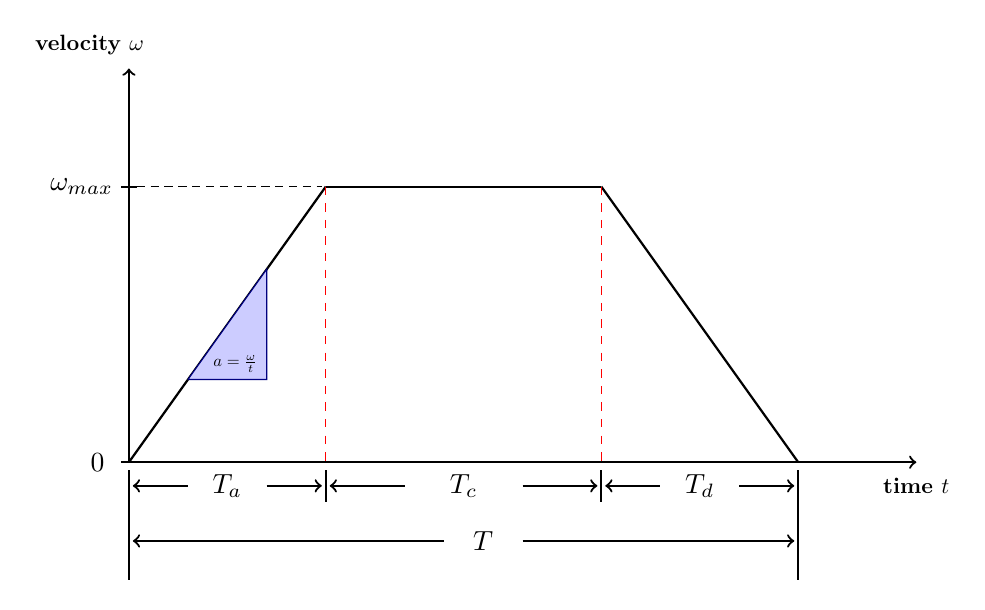
\begin{tikzpicture}
% draw coordinate system
\draw[->,thick] (0,0) -- (10,0);
\draw (10,-0.3) node[scale=0.8] {\textbf{time $t$}};
\draw[->,thick] (0,0) -- (0,5);
\draw[thick] (-0.5,5.3) node[scale=0.8] {\textbf{velocity $\omega$}};
% draw trapezoid
\draw[thick] (0,0) -- (2.5,3.5);
\draw[thick] (2.5,3.5) -- (6,3.5);
\draw[thick] (6,3.5) -- (8.5,0);
% draw acceleration
\filldraw[fill=blue!20!white, draw=blue!50!black] (0.75,1.05) -- (1.75,1.05) -- (1.75,2.45) -- (0.75,1.05);
\draw[black] (1.35,1.25) node[scale=0.6] {$a = \frac{\omega}{t}$};
% draw phase dividers
\draw[red,dashed] (2.5,3.5) -- (2.5,0);
\draw[red,dashed] (6,3.5) -- (6,0);
% draw phase description
\draw (-0.4,0) node {$0$};
\draw[thick] (-0.1,0) -- (0.1,0);
\draw (-0.6,3.5) node {$\omega_{max}$};
\draw[thick] (-0.1,3.5) -- (0.1,3.5);
\draw[densely dashed] (0.1,3.5) -- (2.45,3.5);
\draw[thick] (0,-0.1) -- (0,-1.5);
\draw[<-,thick] (0.05,-0.3) -- (0.75,-0.3);
\draw (1.25,-0.3) node {$T_{a}$};
\draw[->,thick] (1.75,-0.3) -- (2.45,-0.3);
\draw[thick] (2.5,-0.1) -- (2.5,-0.5);
\draw[<-,thick] (2.55,-0.3) -- (3.5,-0.3);
\draw (4.25,-0.3) node {$T_{c}$};
\draw[->,thick] (5,-0.3) -- (5.95,-0.3);
\draw[thick] (6,-0.1) -- (6,-0.5);
\draw[<-,thick] (6.05,-0.3) -- (6.75,-0.3);
\draw (7.25,-0.3) node {$T_{d}$};
\draw[->,thick] (7.75,-0.3) -- (8.45,-0.3);
\draw[thick] (8.5,-0.1) -- (8.5,-1.5);
\draw[<-,thick] (0.05,-1) -- (4,-1);
\draw (4.5,-1) node {$T$};
\draw[->,thick] (5,-1) -- (8.45,-1);
\end{tikzpicture}
\caption{Trapezoidal ramp in detail.}
\label{fig:trapezoid_detail}
\end{figure}
\pagebreak
\subsection{The velocity $\omega$}
Due to the fact, that we have a constant increase in velocity respectively constant acceleration, we can use the standard physics formula for constant acceleration $a$ during $T_{a}$, which is as follows:
\begin{equation}\tag{\textbf{Equation 1}}\label{eq:velocity_trap}
\omega(t) = a \cdot t
\end{equation}
\subsection{Calculation of motor shaft angle $\theta$}
In order to get the position of the motor at a certain point in time, we have to integrate \eqref{eq:velocity_trap}. See Figure \ref{fig:trapezoid_int} for detail.
\newline
\begin{figure}[h]
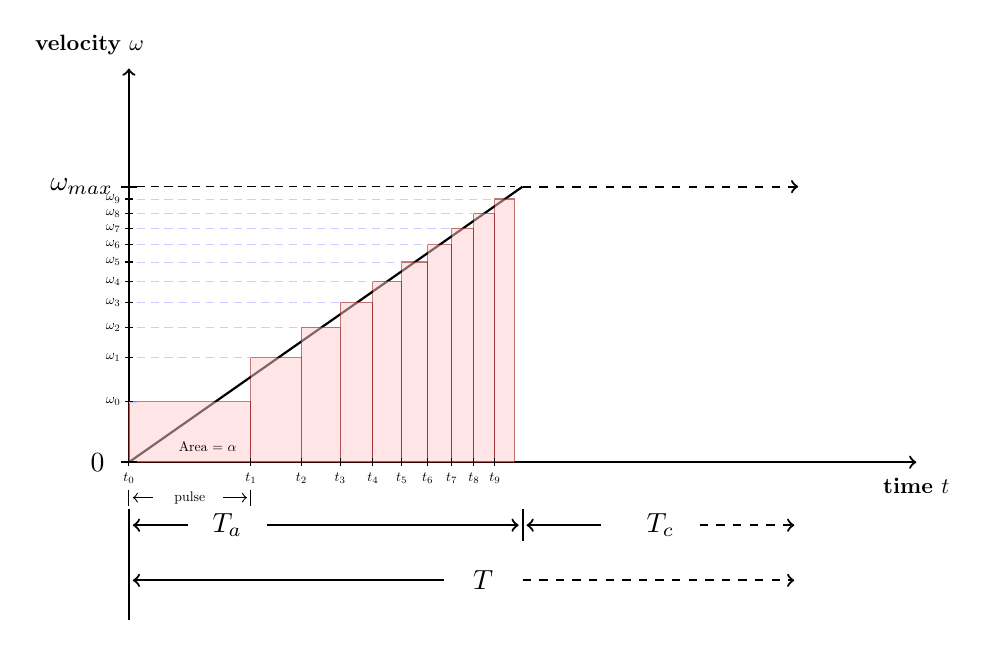
\begin{tikzpicture}
% draw coordinate system
\draw[->,thick] (0,0) -- (10,0);
\draw (10,-0.3) node[scale=0.8] {\textbf{time $t$}};
\draw[->,thick] (0,0) -- (0,5);
\draw[thick] (-0.5,5.3) node[scale=0.8] {\textbf{velocity $\omega$}};
% draw trapezoid
\draw[thick] (0,0) -- (5,3.5);
\draw[->,thick,dashed] (5,3.5) -- (8.5,3.5);
%\draw[thick] (2.5,3.5) -- (6,3.5);
%\draw[thick] (6,3.5) -- (8.5,0);
% draw integral areas
\foreach \x in {0,...,9}{
	\filldraw[fill=red!20!white, draw=red!50!black,opacity=0.5] ({2*sqrt(0.6*\x)},0) rectangle ({2*sqrt(0.6*(\x+1)},{2*sqrt(0.6*(\x+0.5))*0.7});
	\draw ({2*sqrt(0.6*\x)},0.05) -- ({2*sqrt(0.6*\x)},-0.05);
	\draw ({2*sqrt(0.6*\x)},-0.2) node[scale=0.5] {$t_{\x}$};
	\draw (-0.05,{2*sqrt(0.6*(\x+0.5))*0.7}) -- (0.05,{2*sqrt(0.6*(\x+0.5))*0.7});
	\draw (-0.2,{2*sqrt(0.6*(\x+0.5))*0.7}) node[scale=0.5] {$\omega_{\x}$};
	\draw[blue!20!white,very thin,densely dashed] (0.1,{2*sqrt(0.6*(\x+0.5))*0.7}) -- ({2*sqrt(0.6*\x)},{2*sqrt(0.6*(\x+0.5))*0.7});
}
% draw phase description
\draw (-0.4,0) node {$0$};
\draw[thick] (-0.1,0) -- (0.1,0);
\draw (-0.6,3.5) node {$\omega_{max}$};
\draw[thick] (-0.1,3.5) -- (0.1,3.5);
\draw[densely dashed] (0.1,3.5) -- (4.9,3.5);
\draw (1, 0.2) node[scale=0.5] {Area = $\alpha$};
% draw x axis labels
\draw (0,-0.35) -- (0,-0.55);
\draw[<-] (0.05,-0.45) -- (0.3,-0.45);
\draw ({2*sqrt(0.6*0.25)},-0.45) node[scale=0.5] {pulse};
\draw[->] ({2*sqrt(0.6)-0.35},-0.45) -- ({2*sqrt(0.6)-0.05},-0.45);
\draw ({2*sqrt(0.6)},-0.35) -- ({2*sqrt(0.6)},-0.55);
% draw T periods
\draw[thick] (0,-0.6) -- (0,-2);
\draw[<-,thick] (0.05,-0.8) -- (0.75,-0.8);
\draw (1.25,-0.8) node {$T_{a}$};
\draw[->,thick] (1.75,-0.8) -- (4.95,-0.8);
\draw[thick] (5,-0.6) -- (5,-1);
\draw[<-,thick] (5.05,-0.8) -- (6,-0.8);
\draw (6.75,-0.8) node {$T_{c}$};
\draw[->,thick,dashed] (7.25,-0.8) -- (8.45,-0.8);
\draw[<-,thick] (0.05,-1.5) -- (4,-1.5);
\draw (4.5,-1.5) node {$T$};
\draw[->,thick,dashed] (5,-1.5) -- (8.45,-1.5);
\end{tikzpicture}
\caption{Ramp geometry showing n=10 steps.}
\label{fig:trapezoid_int}
\end{figure}
\newline
\newline
\begin{equation}\tag{\textbf{Equation 2}}\label{eq:shaftangle_trap}
\theta(t) = \int_{0}^{t} \omega(\tau)d\tau = \frac{a \cdot t^2}{2} = n \cdot \alpha
\end{equation}
\newline
where $n$  $\geq$ 1 is the step number and $\alpha$ the step angle in radians.
\newline
\newline
\subsection{Calculation of timer delay $t_{n}$}
To get the time point of step number $n$, we need to solve \eqref{eq:shaftangle_trap} for $t$:
\begin{equation}\tag{\textbf{Equation 3}}
t_{n} = \sqrt{\frac{2 \cdot n \cdot \alpha}{a}}
\end{equation}
To get the timer delay between two time points $t_{n+1}$ and $t_{n}$, we just subtract them from one another:
\begin{equation}\tag{\textbf{Equation 4}}
c_{n} = t_{n+1} - t_{n}
\end{equation}
\subsection{Calculation of the number of steps $n$}
Lastly, we need to calculate the number of steps, which are necessary to reach maximum velocity. We do that by combining \eqref{eq:velocity_trap} and \eqref{eq:shaftangle_trap}.
\newline
\newline
From \eqref{eq:velocity_trap} we do get:
\begin{equation*}
t = \frac{\omega}{a}
\end{equation*}
\newline
Inserting this into \eqref{eq:shaftangle_trap}:
\begin{equation*}
\frac{a \cdot \left(\frac{\omega}{a}\right)^2}{2} = n \cdot \alpha
\end{equation*}
\newline
And solving for $n$:
\begin{equation}\tag{\textbf{Equation 5}}
n = \frac{\omega^2}{2 \cdot \alpha \cdot a}
\end{equation}
\pagebreak
\section{S-shaped speed ramp}
In general, trapezoidal ramp profiles (Fig. \ref{fig:trapezoid_detail}) are used for stepper motor acceleration. The problem using trapezoidal ramp profiles is that the system experiences full acceleration right from the beginning, which can either lead to misstepping (signal does not last long enough for the stepper motor to execute a single step) or reaching a lower maximum speed. To prevent this behavior we can use a S-shaped ramp profile (Fig. \ref{fig:sigmoid_detail}). S-shaped profiles consist of a concave period and a convex period. During the concave period acceleration increases to a certain point, also called the inflection point, and then slowly decreases during concave period until maximum velocity is reached. Therefore the system experiences maximum acceleration at the inflection point.
\newline
\newline
\begin{figure}[h]
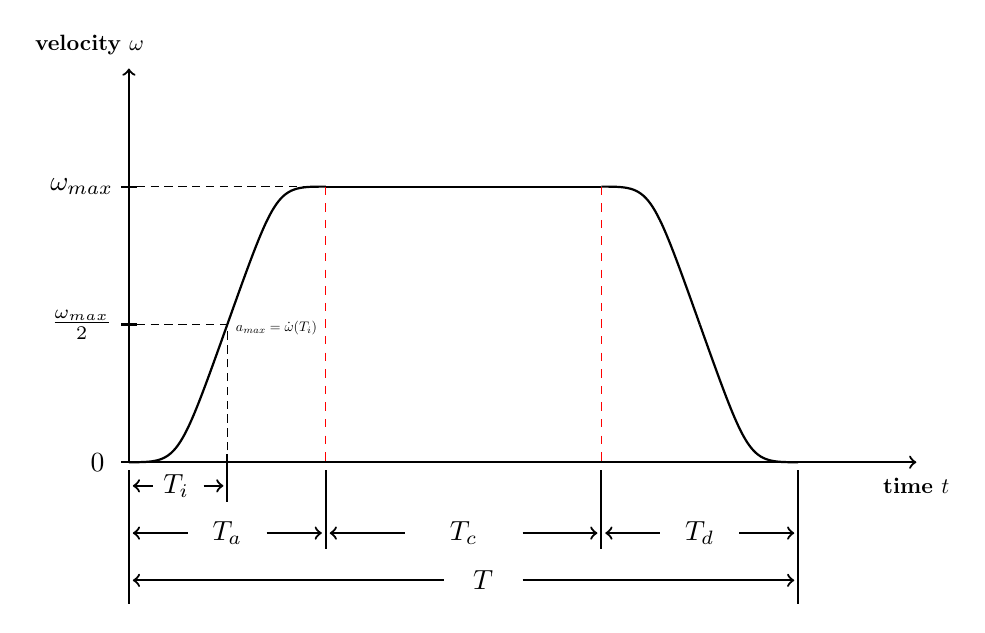
\begin{tikzpicture}
% draw coordinate system
\draw[->,thick] (0,0) -- (10,0);
\draw (10,-0.3) node[scale=0.8] {\textbf{time $t$}};
\draw[->,thick] (0,0) -- (0,5);
\draw[thick] (-0.5,5.3) node[scale=0.8] {\textbf{velocity $\omega$}};
% draw sigmoid
\draw[thick] (0,0) .. controls (0.625,0) .. (1.25,1.75);
\draw[thick] (1.25,1.75) .. controls (1.875,3.5) .. (2.5,3.5);
\draw[thick] (2.5,3.5) -- (6,3.5);
\draw[thick] (6,3.5) .. controls (6.625,3.5) .. (7.25,1.75);
\draw[thick] (7.25,1.75) .. controls (7.875,0) .. (8.5,0);
% draw acceleration
\draw[black] (1.875,1.7) node[scale=0.5] {$a_{max} = \dot{\omega}(T_{i})$};
% draw phase dividers
\draw[red,dashed] (2.5,3.5) -- (2.5,0);
\draw[red,dashed] (6,3.5) -- (6,0);
% draw phase description
\draw (-0.4,0) node {$0$};
\draw[thick] (-0.1,0) -- (0.1,0);
\draw (-0.6,1.75) node {$\frac{\omega_{max}}{2}$};
\draw[thick] (-0.1,1.75) -- (0.1,1.75);
\draw[densely dashed] (0.1,1.75) -- (1.25,1.75);
\draw[thick] (1.25,-0.5) -- (1.25,0.1);
\draw[densely dashed] (1.25,0.15) -- (1.25,1.75);
\draw (-0.6,3.5) node {$\omega_{max}$};
\draw[thick] (-0.1,3.5) -- (0.1,3.5);
\draw[densely dashed] (0.1,3.5) -- (2.45,3.5);
% Draw time periods T
\draw[thick] (0,-0.1) -- (0,-1.8);
%
\draw[<-,thick] (0.05,-0.3) -- (0.3,-0.3);
\draw (0.6,-0.3) node {$T_{i}$};
\draw[->,thick] (0.95,-0.3) -- (1.2,-0.3);
%
%\draw[<-,thick] (1.3,-0.3) -- (1.6,-0.3);
%\draw (1.9,-0.3) node {$T_{cx}$};
%\draw[->,thick] (2.15,-0.3) -- (2.45,-0.3);
%
\draw[<-,thick] (0.05,-0.9) -- (0.75,-0.9);
\draw (1.25,-0.9) node {$T_{a}$};
\draw[->,thick] (1.75,-0.9) -- (2.45,-0.9);
\draw[thick] (2.5,-0.1) -- (2.5,-1.1);
\draw[<-,thick] (2.55,-0.9) -- (3.5,-0.9);
\draw (4.25,-0.9) node {$T_{c}$};
\draw[->,thick] (5,-0.9) -- (5.95,-0.9);
\draw[thick] (6,-0.1) -- (6,-1.1);
\draw[<-,thick] (6.05,-0.9) -- (6.75,-0.9);
\draw (7.25,-0.9) node {$T_{d}$};
\draw[->,thick] (7.75,-0.9) -- (8.45,-0.9);
\draw[thick] (8.5,-0.1) -- (8.5,-1.8);
\draw[<-,thick] (0.05,-1.5) -- (4,-1.5);
\draw (4.5,-1.5) node {$T$};
\draw[->,thick] (5,-1.5) -- (8.45,-1.5);
\end{tikzpicture}
\caption{S-shaped ramp in detail.}
\label{fig:sigmoid_detail}
\end{figure}
\newline
\newline
To represent the S-shaped acceleration profile ($0 \leq t \leq T_{a}$) we can use a special case of a sigmoid function, the logistic function, which has the form:
\begin{equation*}
S(t) = \frac{1}{1+\mathrm{e}^{-t}}
\end{equation*}
\subsection{Finding a suitable velocity function $\omega$}
To be able to use this function, we have to modify it to meet certain criteria:
\begin{align*}
S(T_{a}) = \omega_{max} & \\
S(T_{i}) = \frac{\omega_{max}}{2} & \\
\dot{S}(T_{i}) = a_{max}
\end{align*}
\newline
where $T_{i}$ is the time period to the inflection point, $T_{a}$ is the total acceleration period and $\omega_{max}$ is the maximum velocity.
\newline
\newline
Using this criteria we can generate a final modified version of the logistic function to represent velocity $\omega$ on a S-shaped ramp profile:
\begin{equation}\tag{\textbf{Equation 1}}\label{eq:velocity}
\omega(\tau) = \frac{\omega}{\mathrm{e}^{\left(\frac{4 \cdot a}{\omega}\right) \cdot \left(T_{i} - \tau\right)}+1}
\end{equation}
\newline
where $\omega$ is the maximum velocity and $a$ is the maximum acceleration (respectively the acceleration at the inflection point $T_{i}$) that can be reached.
\subsection{Calculation of motor shaft angle $\theta$}
Integration of $\omega(\tau)$ gives the motor shaft angle $\theta$($t$):
%
\begin{equation}\tag{\textbf{Equation 2}}\label{eq:shaftangle}
\theta(t) = \int_{0}^{t} \omega(\tau)d\tau = \dfrac{\omega^2\left(\ln\left(\mathrm{e}^\frac{4 \cdot a \cdot t}{\omega}+\mathrm{e}^\frac{4 \cdot a \cdot T_{i}}{\omega}\right)-\ln\left(\mathrm{e}^\frac{4 \cdot a \cdot T_{i}}{\omega}+1\right)\right)}{4 \cdot a} = n \cdot \alpha
\end{equation}
\newline
where $n$  $\geq$ 1 is the step number and $\alpha$ the step angle in radians.
\newline
\newline
\subsection{Calculation of timer delay $t_{n}$}
To get an exact timer delay (pulse width) for the stepper motor STEP signal, we need to solve \eqref{eq:shaftangle} for $t$:
\begin{align*}
\dfrac{\omega^2\left(\ln\left(\mathrm{e}^\frac{4 \cdot a \cdot t}{\omega}+\mathrm{e}^\frac{4 \cdot a \cdot T_{i}}{\omega}\right)-\ln\left(\mathrm{e}^\frac{4 \cdot a \cdot T_{i}}{\omega}+1\right)\right)}{4 \cdot a} &= n \cdot \alpha & \\
\ln\left(\mathrm{e}^\frac{4 \cdot a \cdot t}{\omega}+\mathrm{e}^\frac{4 \cdot a \cdot T_{i}}{\omega}\right)-\ln\left(\mathrm{e}^\frac{4 \cdot a \cdot T_{i}}{\omega}+1\right) &= \frac{4 \cdot a \cdot n \cdot \alpha}{\omega^2} & \\
\ln\left(\dfrac{\mathrm{e}^\frac{4 \cdot a \cdot t}{\omega}+\mathrm{e}^\frac{4 \cdot a \cdot T_{i}}{\omega}}{\mathrm{e}^\frac{4 \cdot a \cdot T_{i}}{\omega}+1}\right) &= \frac{4 \cdot a \cdot n \cdot \alpha}{\omega^2} & \\
\mathrm{e}^{\ln\left(\dfrac{\mathrm{e}^\frac{4 \cdot a \cdot t}{\omega}+\mathrm{e}^\frac{4 \cdot a \cdot T_{i}}{\omega}}{\mathrm{e}^\frac{4 \cdot a \cdot T_{i}}{\omega}+1}\right)} &= \mathrm{e}^{\frac{4 \cdot a \cdot n \cdot \alpha}{\omega^2}} & \\
\dfrac{\mathrm{e}^\frac{4 \cdot a \cdot t}{\omega}+\mathrm{e}^\frac{4 \cdot a \cdot T_{i}}{\omega}}{\mathrm{e}^\frac{4 \cdot a \cdot T_{i}}{\omega}+1} &= \mathrm{e}^{\frac{4 \cdot a \cdot n \cdot \alpha}{\omega^2}} & \\
\mathrm{e}^\frac{4 \cdot a \cdot t}{\omega} &= \left(\mathrm{e}^\frac{4 \cdot a \cdot T_{i}}{\omega}+1\right) \left(\mathrm{e}^{\frac{4 \cdot a \cdot n \cdot \alpha}{\omega^2}}\right) - \mathrm{e}^\frac{4 \cdot a \cdot T_{i}}{\omega} & \\
\ln\left(\mathrm{e}^\frac{4 \cdot a \cdot t}{\omega}\right) &= \ln\left(\left(\mathrm{e}^\frac{4 \cdot a \cdot T_{i}}{\omega}+1\right) \left(\mathrm{e}^{\frac{4 \cdot a \cdot n \cdot \alpha}{\omega^2}}\right) - \mathrm{e}^\frac{4 \cdot a \cdot T_{i}}{\omega}\right) & \\
\frac{4 \cdot a \cdot t}{\omega} &= \ln\left(\left(\mathrm{e}^\frac{4 \cdot a \cdot T_{i}}{\omega}+1\right) \left(\mathrm{e}^{\frac{4 \cdot a \cdot n \cdot \alpha}{\omega^2}}\right) - \mathrm{e}^\frac{4 \cdot a \cdot T_{i}}{\omega}\right) & \\
t &= \omega \frac{\ln\left(\left(\mathrm{e}^\frac{4 \cdot a \cdot T_{i}}{\omega}+1\right) \left(\mathrm{e}^{\frac{4 \cdot a \cdot n \cdot \alpha}{\omega^2}}\right) - \mathrm{e}^\frac{4 \cdot a \cdot T_{i}}{\omega}\right)}{4 \cdot a}
\end{align*}
\newline
After simplification we obtain:
%
\begin{equation}\tag{\textbf{Equation 3}}\label{eq:tn}
t_{n} = \omega \frac{\ln\left(\left(\mathrm{e}^\frac{4 \cdot a \cdot T_{i}}{\omega}+1\right) \cdot \left(\mathrm{e}^{\frac{4 \cdot a \cdot n \cdot \alpha}{\omega^2}}\right) - \mathrm{e}^\frac{4 \cdot a \cdot T_{i}}{\omega}\right)}{4 \cdot a}
\end{equation}
\newline
The exact delay between the $n$-th and $(n+1)$-th step pulse can then be calculated as follows:
%
\begin{equation}\tag{\textbf{Equation 4}}\label{eq:cn}
c_{n} = t_{n+1} - t_{n}
\end{equation}
%
\subsection{Calculating the number of steps $n$}
Finally, we need to calculate the number of steps that are necessary for the stepper motor to reach maximum velocity. As our defined velocity function (see \eqref{eq:velocity})only reaches its maximum value while $t$ being infinity, we increase the maximum velocity $\omega$ by 0.5\% to get a finite number of steps. We can combine \eqref{eq:velocity} and \eqref{eq:shaftangle} to get the number of steps. 
\newline
\newline
Solving \eqref{eq:velocity} for $t$, we get:
\begin{equation*}
t = T_{i} - \frac{\ln\left(1.005 \cdot \omega-1\right)}{\frac{4 \cdot a}{\omega}}
\end{equation*}
\newline
Now we can insert $t$ into \eqref{eq:shaftangle} and obtain:
\begin{equation}\tag{\textbf{Equation 5}}\label{eq:nsteps}
n = \dfrac{\omega^2\left(\ln\left(\mathrm{e}^\frac{4 \cdot a \cdot \left(T_{i} - \frac{\ln\left(\frac{\omega}{0.995 \cdot \omega}-1\right)}{\frac{4 \cdot a}{\omega}}\right)}{\omega}+\mathrm{e}^\frac{4 \cdot a \cdot T_{i}}{\omega}\right)-\ln\left(\mathrm{e}^\frac{4 \cdot a \cdot T_{i}}{\omega}+1\right)\right)}{4 \cdot a \cdot \alpha}
\end{equation}
\pagebreak
\section{Implementation}
\subsection{Pseudocode}
Next, we want to see how such a motion profile of a stepper motor can be implemented. Therefore, we have this pseudocode snippet:
\begin{algorithm}
	\caption{Calculate ramp profile}
	\begin{algorithmic}[1]
		\State $c\gets$ empty list
		\State $n \gets calculateNumberOfSteps()$
		\State $i \gets 0$
		\While{$i < n$}
			\State $t_\text{n+1} \gets calculateT(n+1)$
			\State $t_\text{n} \gets calculateT(n)$
			\State $c_\text{n} \gets t_\text{n+1} - t_\text{n}$
			\State $c[i]\gets c_\text{n}$
			\State $i \gets i + 1$
		\EndWhile
	\end{algorithmic}
\end{algorithm}
\subsection{Implementation in Python}
Below is an implementation example of a trapezoidal speed ramp in Python.
\begin{lstlisting}[language=Python, caption=Python example of trapezodial speed ramp calculation]
import math

step_angle = 1.8    # Step Angle of stepper motor in degrees
microsteps = 2      # Microstepping mode
travel_per_rev = 5  # Axis travel per stepper motor revolution
accel = 80.0        # Acceleration in [mm/s^2]

sqrt = math.sqrt
spr = 360.0 / step_angle * microsteps
steps_per_mm = spr / travel_per_rev
step_angle_in_rad = 2 * math.pi / spr
cf = vm / 60 * steps_per_mm * step_angle_in_rad
accel_fact = accel * steps_per_mm * step_angle_in_rad
num_steps = int(round(cf * cf / (2 * step_angle_in_rad * accel_fact)))
c0 = sqrt(2 * step_angle_in_rad / accel_fact)
c = [c0]
for i in range(1, num_steps):
	cn = c0 * (sqrt(i+1) - sqrt(i))
	c.append(cn)
c_total = sum(c)
\end{lstlisting}
Next, we have an implementation example of a sigmoidal acceleration ramp in Python.
\newline
\begin{lstlisting}[language=Python, caption=Python example of sigmoidal speed ramp calculation]
import math

step_angle = 1.8    # Step Angle of stepper motor in degrees
microsteps = 2      # Microstepping mode
travel_per_rev = 5  # Axis travel per stepper motor revolution
accel = 80.0        # Acceleration in [mm/s^2]

sqrt = math.sqrt
spr = 360.0 / step_angle * microsteps
steps_per_mm = spr / travel_per_rev
step_angle_in_rad = 2 * math.pi / spr
cf = vm / 60 * steps_per_mm * step_angle_in_rad
accel_fact = accel * steps_per_mm * step_angle_in_rad

T_2 = 0.4
# pre-calculated values
a_func = math.e**(4 * accel_fact * T_2 / cf)
t_tmp = T_2 - math.log(cf/(0.995*cf)-1)/(4*accel_fact/cf)

num_steps = int(round(cf**2 * (math.log(math.e**(4*accel_fact*t_tmp/cf) + a_func) - math.log(a_func + 1)) / (4 * accel_fact * step_angle_in_rad)))
c = []
for i in range(num_steps):
	cn_i_plus_one = cf * math.log((a_func + 1) * (math.e**(4 * accel_fact * (i+1) * step_angle_in_rad / cf**2)) - a_func) / (4 * accel_fact)
	cn_i = cf * math.log((a_func + 1) * (math.e**(4 * accel_fact * i * step_angle_in_rad / cf**2)) - a_func) / (4 * accel_fact)
	cn = cn_i_plus_one - cn_i
	c.append(cn)
c_total = sum(c)
\end{lstlisting}
\pagebreak
\subsection{Output}
Below are some examples of calculated profiles with the code above. Every point represents a step signal.
\newline
\begin{figure}[h]
	\begin{subfigure}[b]{0.5\linewidth}
		\includegraphics[width=\linewidth]{ramp_profile_t50mm.jpg}
		\caption{trapezoidal}
		\label{fig:profile1}
	\end{subfigure}
	\begin{subfigure}[b]{0.5\linewidth}
		\includegraphics[width=\linewidth]{ramp_profile_s50mm.jpg}
		\caption{S-shaped}
		\label{fig:profile2}
	\end{subfigure}
	\caption{Comparison of ramp profiles.}
\end{figure}
%
\end{document}  